% Name: Row reduction of an augmented matrix
% Description: The augmented matrix of a system of three equations and the row operations, written beside it, that take it a step toward echelon form.
% Tags: augmented matrix, row reduction, Gaussian elimination, linear systems

\usetikzlibrary{arrows.meta, positioning}

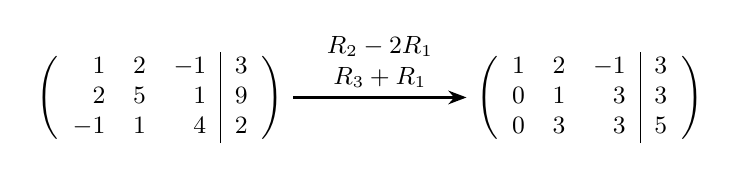
\begin{tikzpicture}[>={Stealth}, every node/.style={font=\small}]
  \node (A) {$\left(\begin{array}{rrr|r} 1 & 2 & -1 & 3 \\ 2 & 5 & 1 & 9 \\ -1 & 1 & 4 & 2 \end{array}\right)$};
  \node[right=2.2cm of A] (B) {$\left(\begin{array}{rrr|r} 1 & 2 & -1 & 3 \\ 0 & 1 & 3 & 3 \\ 0 & 3 & 3 & 5 \end{array}\right)$};
  \draw[->, thick] (A) -- (B) node[midway, above, align=center] {$R_2 - 2R_1$ \\ $R_3 + R_1$};
\end{tikzpicture}
